\subsection{Correctness}
The souffle pretty-printer is used to output a Datalog program that may be evaluated by souffle. The process of comparing the output of souffle to that of the internal interpreter has been automated and a range of tests written. If the tests agree then the souffle pretty-printer is said to be correct for the test program. Given that souffle correctly implements Datalog, the interpreter too is concluded to be correct for the given test program. The test cases are selected to cover mutual recursion, negation, meta-predicates, and the other various language extensions.

\subsection{Performance}
Souffle implements semi-naive evaluation\cite{Green:2013:DRQ:2688167.2688168} which is the same as naive evaluation except that it utilizes the following key-insight. An instantiation of the terms of a rule may derive new tuple(s) if and only if at least one tuple that was derived in the previous iteration is used in the instantiation.
The Nat example with an upper limit of $N$ highlights the difference in performance that this may give.
\begin{minted}{yaml}
Nat(0).
Nat(y) :- Nat(x), BIND(y, x + 1), y <= N.
\end{minted}
\noindent
To evaluate using naive evaluation, in each step with $k$ unary tuples in $Nat$, the evaluation must Select all tuples from Nat, calculate y for each x, filter all calculated y with the less than rule, project the $y$ component into the new Nat relation, and take the union between the old and the new Nat relation. With the current implementation, union has time complexity $O(k \cdot log(k))$ (using an ordered set for the relations) and the remaining operations are $O(k)$. The expected time-complexity for the NAT-example is thus in the order of:
\begin{align*}
\sum_{k = 1}^{N} 4 k + k \cdot log (k) \leq 4 N^2 + N^2 log(N) = O(N^2 log(N))
\end{align*}
For semi-naive evaluation, each iteration gives a single new element to consider. The corresponding time complexity thus reduces to the order of:
\begin{align*}
	\sum_{k = 1}^{N} 4 + log (k) \leq 4N + N log(N) = O(N log(N))
\end{align*}

\subsubsection{Experimental Results}
The NAT example was measured for for inputs in range 100 to 10000 for the internal naive evaluation and for 4096 to 536870912 for souffle that uses semi-naive evaluation. For the naive evaluation, the theoretical results was confirmed as $O(N^2 log(N))$ (see figure \ref{figure:internalloglog}). For souffle semi-naive, the experimental results (see figure \ref{figure:souffleloglog}) show $O(N)$ behavior; souffle uses an index based relation data structure as opposed to an ordered set.

\begin{figure}[!ht]
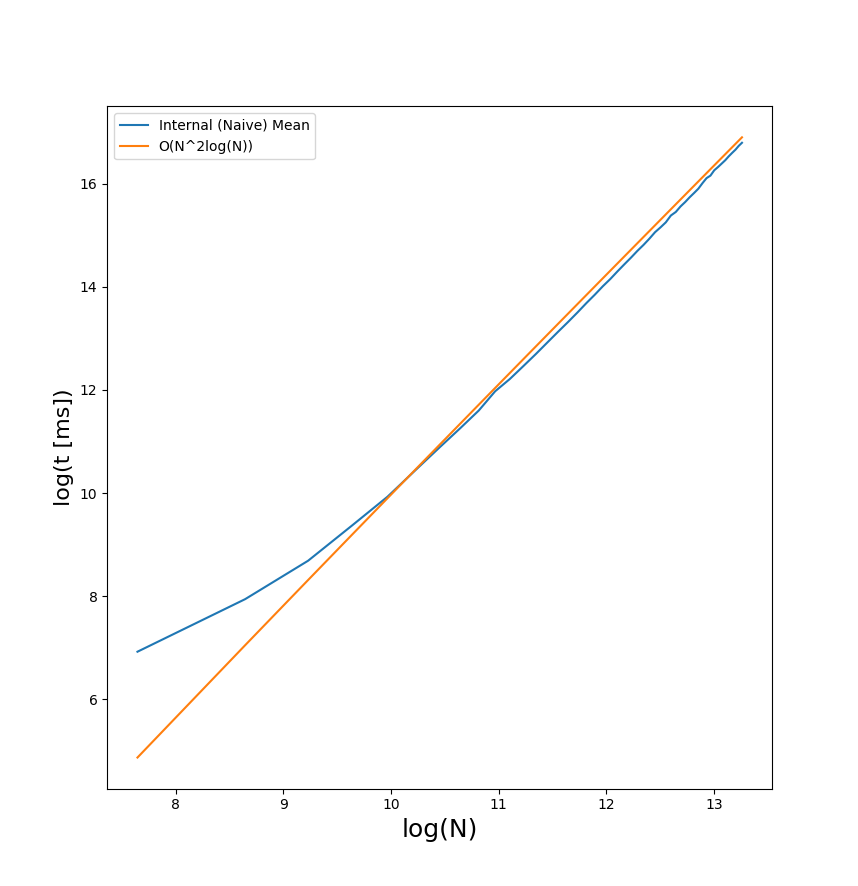
\includegraphics[width=.9\linewidth, height=12\baselineskip]{img/internalloglog.png}
\caption{Log-log plot for the naive evaluation method of the NAT example.}
\label{figure:internalloglog}
\end{figure}

\begin{figure}[!ht]
	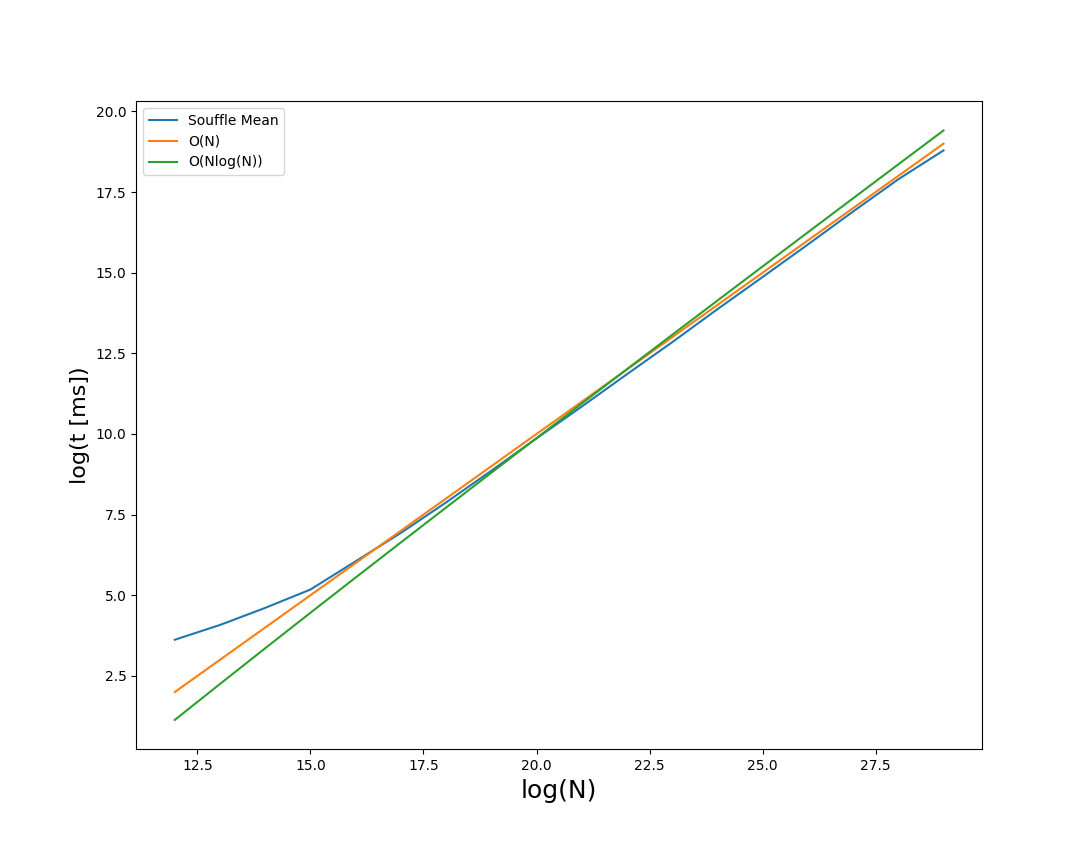
\includegraphics[width=.9\linewidth, height=12\baselineskip]{img/souffleloglog.png}
	\caption{Log-log plot for the souffle semi-naive evaluation method of the NAT example.}
	\label{figure:souffleloglog}
\end{figure}

\subsection{Expressive Power}
\textit{To be Written ... }